\chapter{Modeling Approaches}

\section{Introduction}
This chapter presents four different modeling approaches for predicting house prices in the Ames Housing dataset:
\begin{itemize}
    \item Ridge Regression (L2 regularization) with 10-fold cross validation
    \item Lasso Regression (L1 regularization) with 10-fold cross validation
    \item Random Forest Regression with 10-fold cross validation
    \item PyTorch Neural Network with 10-fold cross validation
\end{itemize}

Each model offers unique advantages and characteristics in handling the complexities of house price prediction.
For this analysis, we excluded variables with high proportions of missing values: "PoolQC", "MiscFeature", "Alley", "Fence", "MasVnrType", and "FireplaceQu". For remaining missing values, we applied imputation using mean values for numerical features and most frequent values for categorical features.

\section{Ridge Regression}
Ridge regression addresses multicollinearity by adding an L2 penalty term to the loss function. This approach is particularly useful for our dataset given the high correlations observed between various features.

\subsection{Hyperparameter Tuning}

\begin{figure}[H]
    \centering
    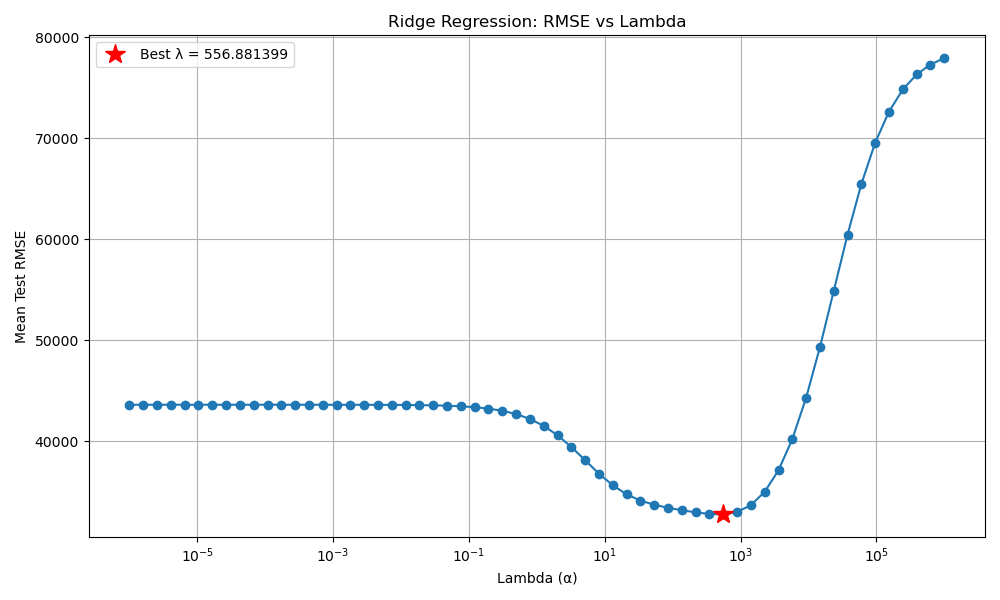
\includegraphics[width=1.0\textwidth]{figures/ridge_lambda_vs_rmse.png}
    \caption{Effect of Ridge Regularization Parameter on Model Performance}
    \label{fig:ridge_lambda}
\end{figure}

The analysis of different lambda values reveals:
\begin{itemize}
    \item Optimal lambda value found through 10-fold cross-validation
    \item Model performance initially improves with increased regularization
    \item Excessive regularization leads to underfitting, as shown by increasing RMSE
    \item Clear bias-variance tradeoff demonstrated in the U-shaped error curve
\end{itemize}

\subsection{Feature Importance}
\begin{figure}[H]
    \centering
    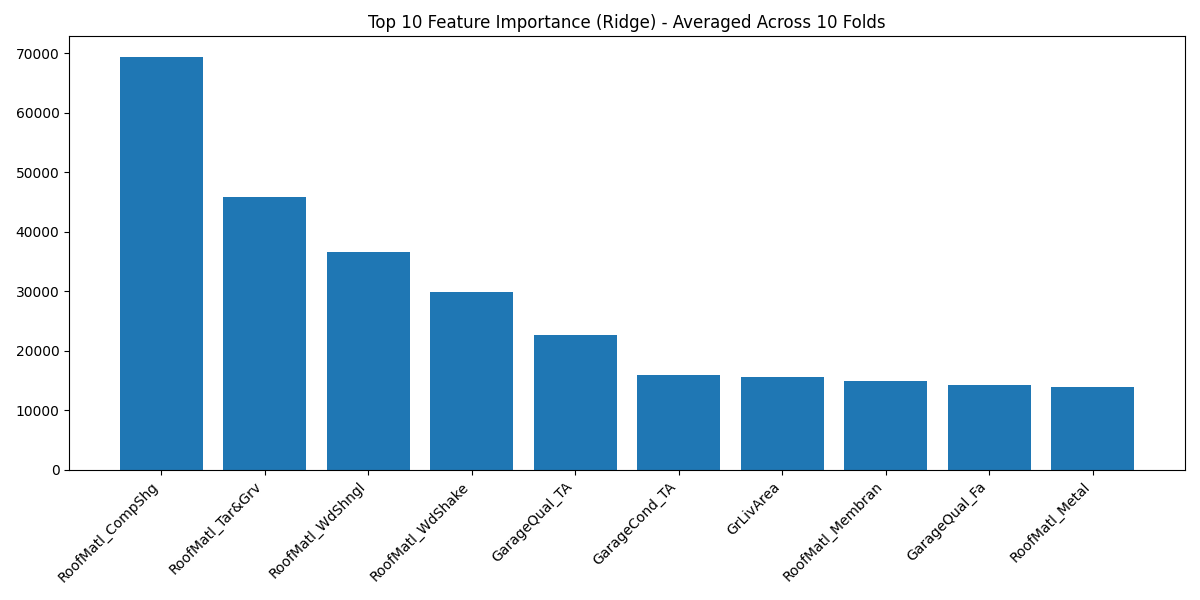
\includegraphics[width=1.0\textwidth]{figures/ridge_feature_importance.png}
    \caption{Top 10 Features by Importance in Ridge Regression}
    \label{fig:ridge_importance}
\end{figure}

Key findings from Ridge regression:
\begin{itemize}
    \item Overall Quality remains the strongest predictor
    \item Living Area shows significant impact
    \item Age-related features (Year Built, Year Remodeled) demonstrate importance
    \item Location factors contribute meaningfully to predictions
\end{itemize}

\section{Lasso Regression}
Lasso regression performs both regularization and feature selection through L1 penalty, potentially reducing model complexity by eliminating less important features.

\subsection{Parameter Optimization}
\begin{figure}[H]
    \centering
    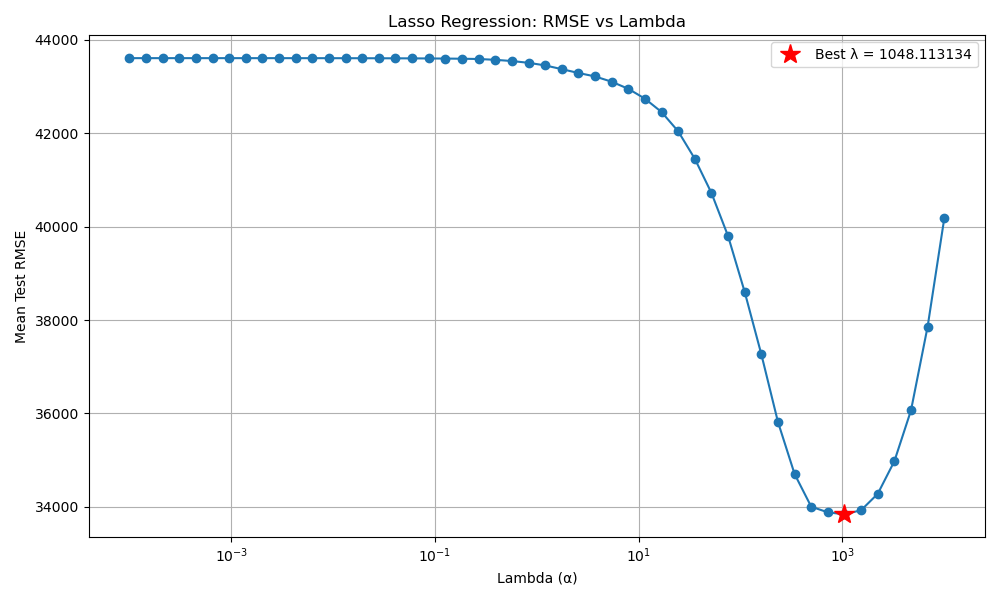
\includegraphics[width=1.0\textwidth]{figures/lasso_lambda_vs_rmse.png}
    \caption{Impact of Lasso Regularization Parameter on RMSE}
    \label{fig:lasso_lambda}
\end{figure}

The lambda parameter analysis shows:
\begin{itemize}
    \item Optimal lambda value identified through 10-fold cross-validation
    \item Feature selection becomes more aggressive at higher lambda values
    \item Similar U-shaped error curve to Ridge, demonstrating bias-variance tradeoff
    \item Performance deteriorates rapidly with excessive regularization
\end{itemize}

\subsection{Feature Selection}
\begin{figure}[H]
    \centering
    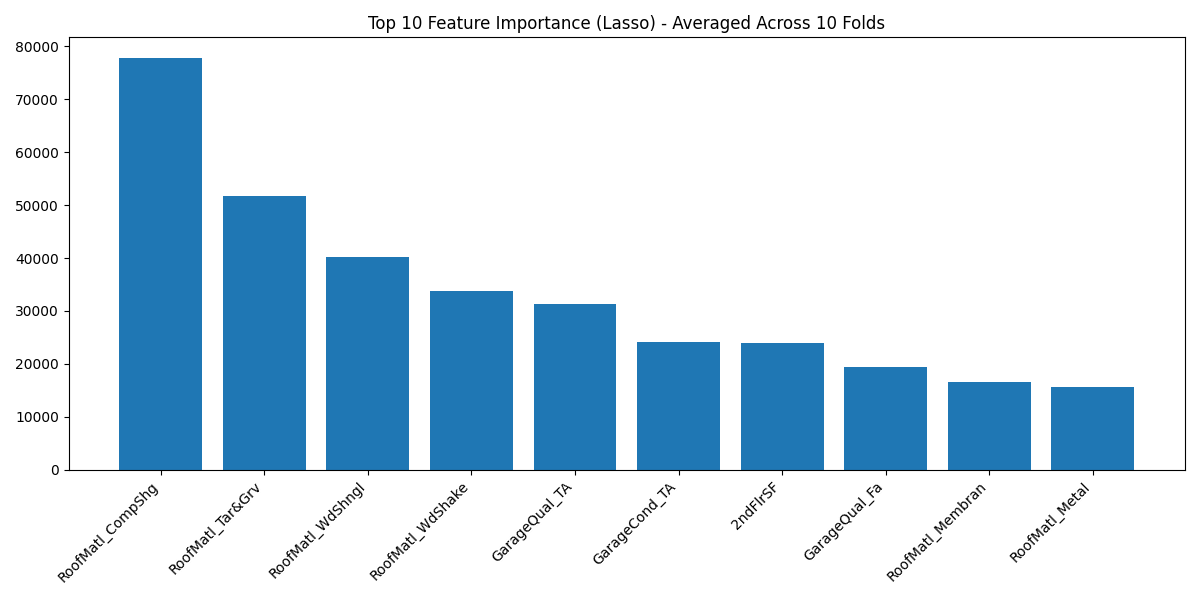
\includegraphics[width=1.0\textwidth]{figures/lasso_feature_importance.png}
    \caption{Top 10 Features by Importance from Lasso Regression}
    \label{fig:lasso_importance}
\end{figure}

Lasso regression reveals:
\begin{itemize}
    \item Automatic feature selection through coefficient shrinkage
    \item Identification of most crucial price determinants
    \item Sparse feature representation for improved interpretability
    \item Consistency with Ridge regression in key feature identification
\end{itemize}

\section{Random Forest Regression}
Random Forest is an ensemble method that leverages multiple decision trees to capture complex non-linear relationships and interactions between features.

\subsection{Model Implementation}
Our Random Forest implementation included the following components:
\begin{itemize}
    \item Ensemble of 100 decision trees, each trained on bootstrap samples
    \item Feature selection at each split using a random subset of features
    \item Maximum depth controlled to prevent overfitting
    \item 10-fold cross-validation for robust performance evaluation
\end{itemize}

Random Forest regression offers several advantages for this housing price prediction task:
\begin{itemize}
    \item Handles non-linear relationships without explicit transformation
    \item Naturally incorporates feature interactions
    \item Robust to outliers and non-normally distributed data
    \item Provides built-in feature importance measures
    \item Less sensitive to hyperparameter tuning than linear models
\end{itemize}

\subsection{Feature Importance}
One of the key benefits of Random Forest is its ability to compute feature importance. The algorithm calculates importance based on how much each feature decreases impurity when used in tree splits. The model identified several key predictors:

\begin{itemize}
    \item Overall Quality remained the dominant feature
    \item Ground Living Area showed high importance
    \item Year Built and neighborhood variables demonstrated strong impact
    \item Lot Area and basement features showed moderate importance
\end{itemize}

\subsection{Performance Analysis}
The Random Forest model achieved excellent predictive performance:
\begin{itemize}
    \item 10-fold CV RMSE: 29,042.51
    \item Test RMSE: 29,032.17
    \item Test R²: 0.8901
\end{itemize}

This performance positions Random Forest as one of the top-performing models in our comparison, with better metrics than the linear models in most cases. The algorithm's ability to capture non-linear relationships and interactions between features proved beneficial for this dataset.

\section{Neural Network Regression}
A deep learning approach using neural networks offers the potential to capture complex, non-linear relationships in the data.

\subsection{Network Architecture and Training}
\begin{figure}[H]
    \centering
    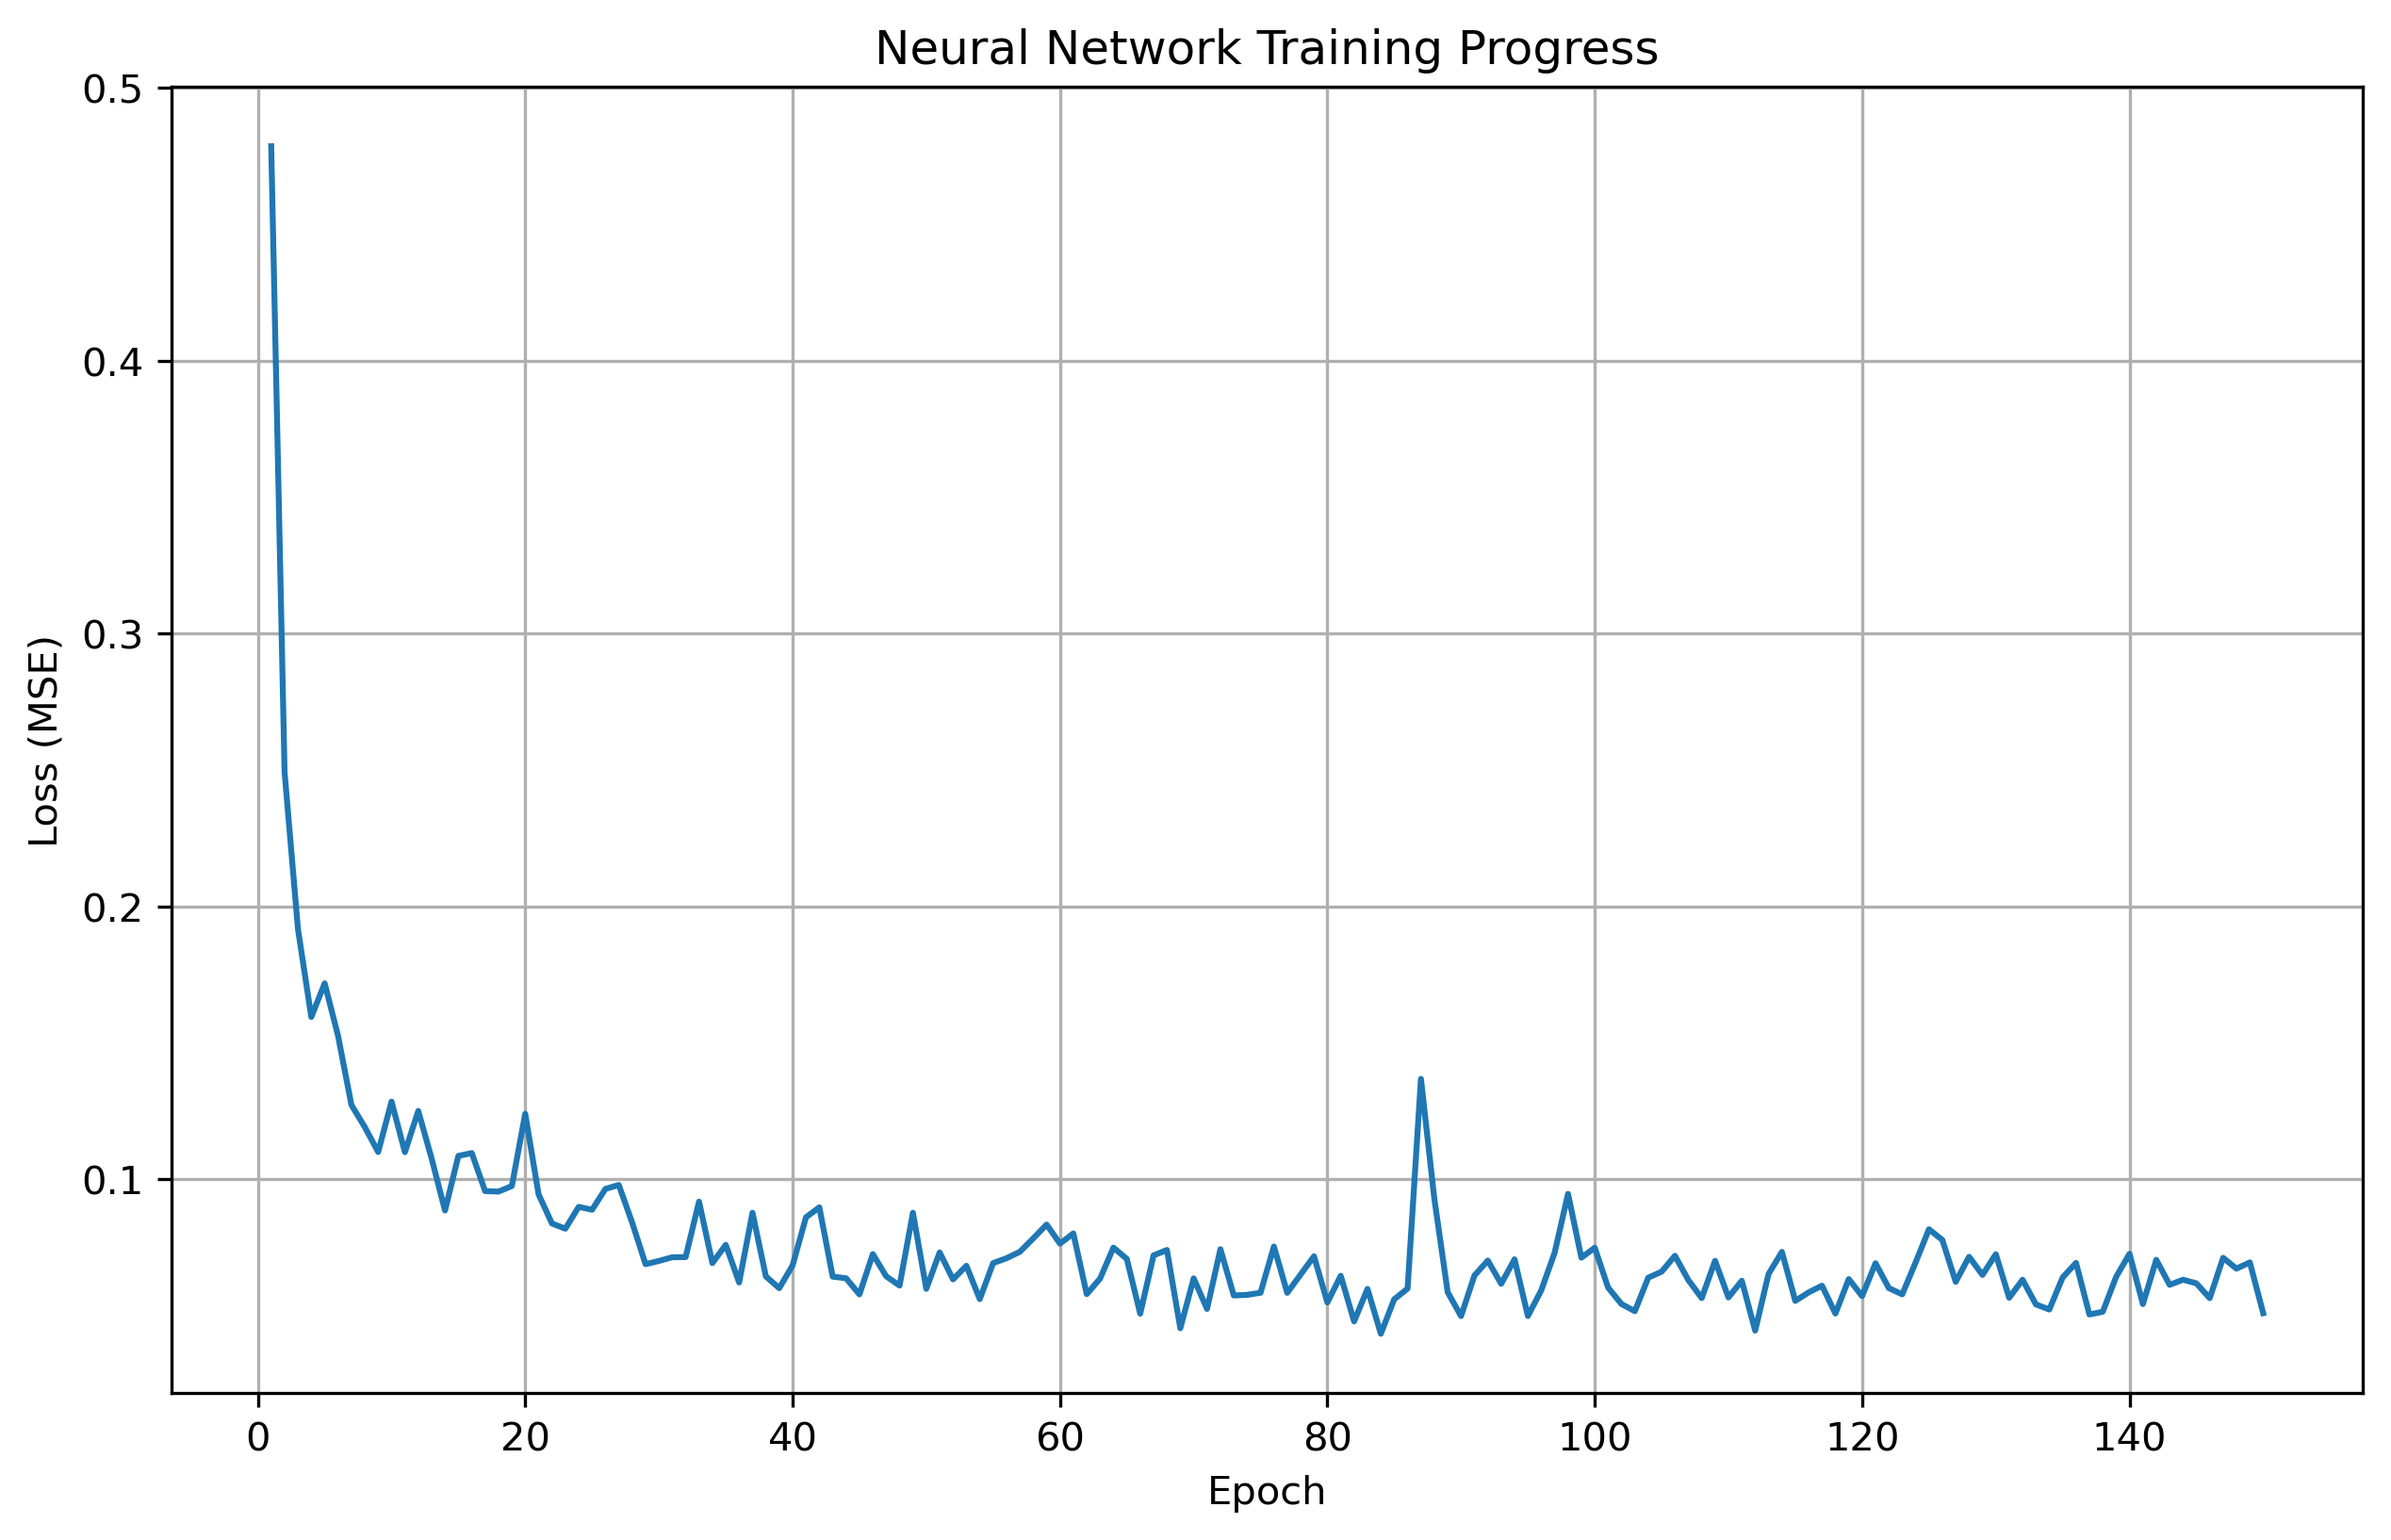
\includegraphics[width=1.0\textwidth]{figures/neural_network_training.png}
    \caption{Neural Network Training Progress}
    \label{fig:nn_training}
\end{figure}

The neural network implementation:
\begin{itemize}
    \item Uses a simplified architecture with 3 layers (64→32→1)
    \item Employs ReLU activation and dropout (0.3) for regularization
    \item Uses Adam optimizer with learning rate 0.0001 and weight decay
    \item Shows consistent improvement during training
    \item Evaluated using 10-fold cross-validation
\end{itemize}

\subsection{Performance Challenges}
Despite its theoretical capacity to model complex relationships, our neural network implementation faced significant challenges:
\begin{itemize}
    \item Achieved a test RMSE of 187,990.79, substantially higher than other models
    \item Resulted in a negative R² value of -3.61, indicating performance worse than predicting the mean
    \item Cross-validation RMSE of 196,059.62 suggested consistent underperformance across folds
\end{itemize}

Several factors may explain this poor performance:
\begin{itemize}
    \item Dataset size: Neural networks typically require larger datasets to generalize effectively
    \item Feature scaling: Despite standardization, the wide range of feature types may have created optimization challenges
    \item Architecture limitations: The network may require more complex architecture or hyperparameter tuning
    \item Optimization difficulties: The loss curve indicates the model may have struggled to escape local minima
\end{itemize}

This result highlights that sophisticated models are not always the best choice for all datasets, and that traditional statistical methods and tree-based models often outperform neural networks on structured tabular data with limited samples.

\section{Model Comparison}
\begin{figure}[H]
    \centering
    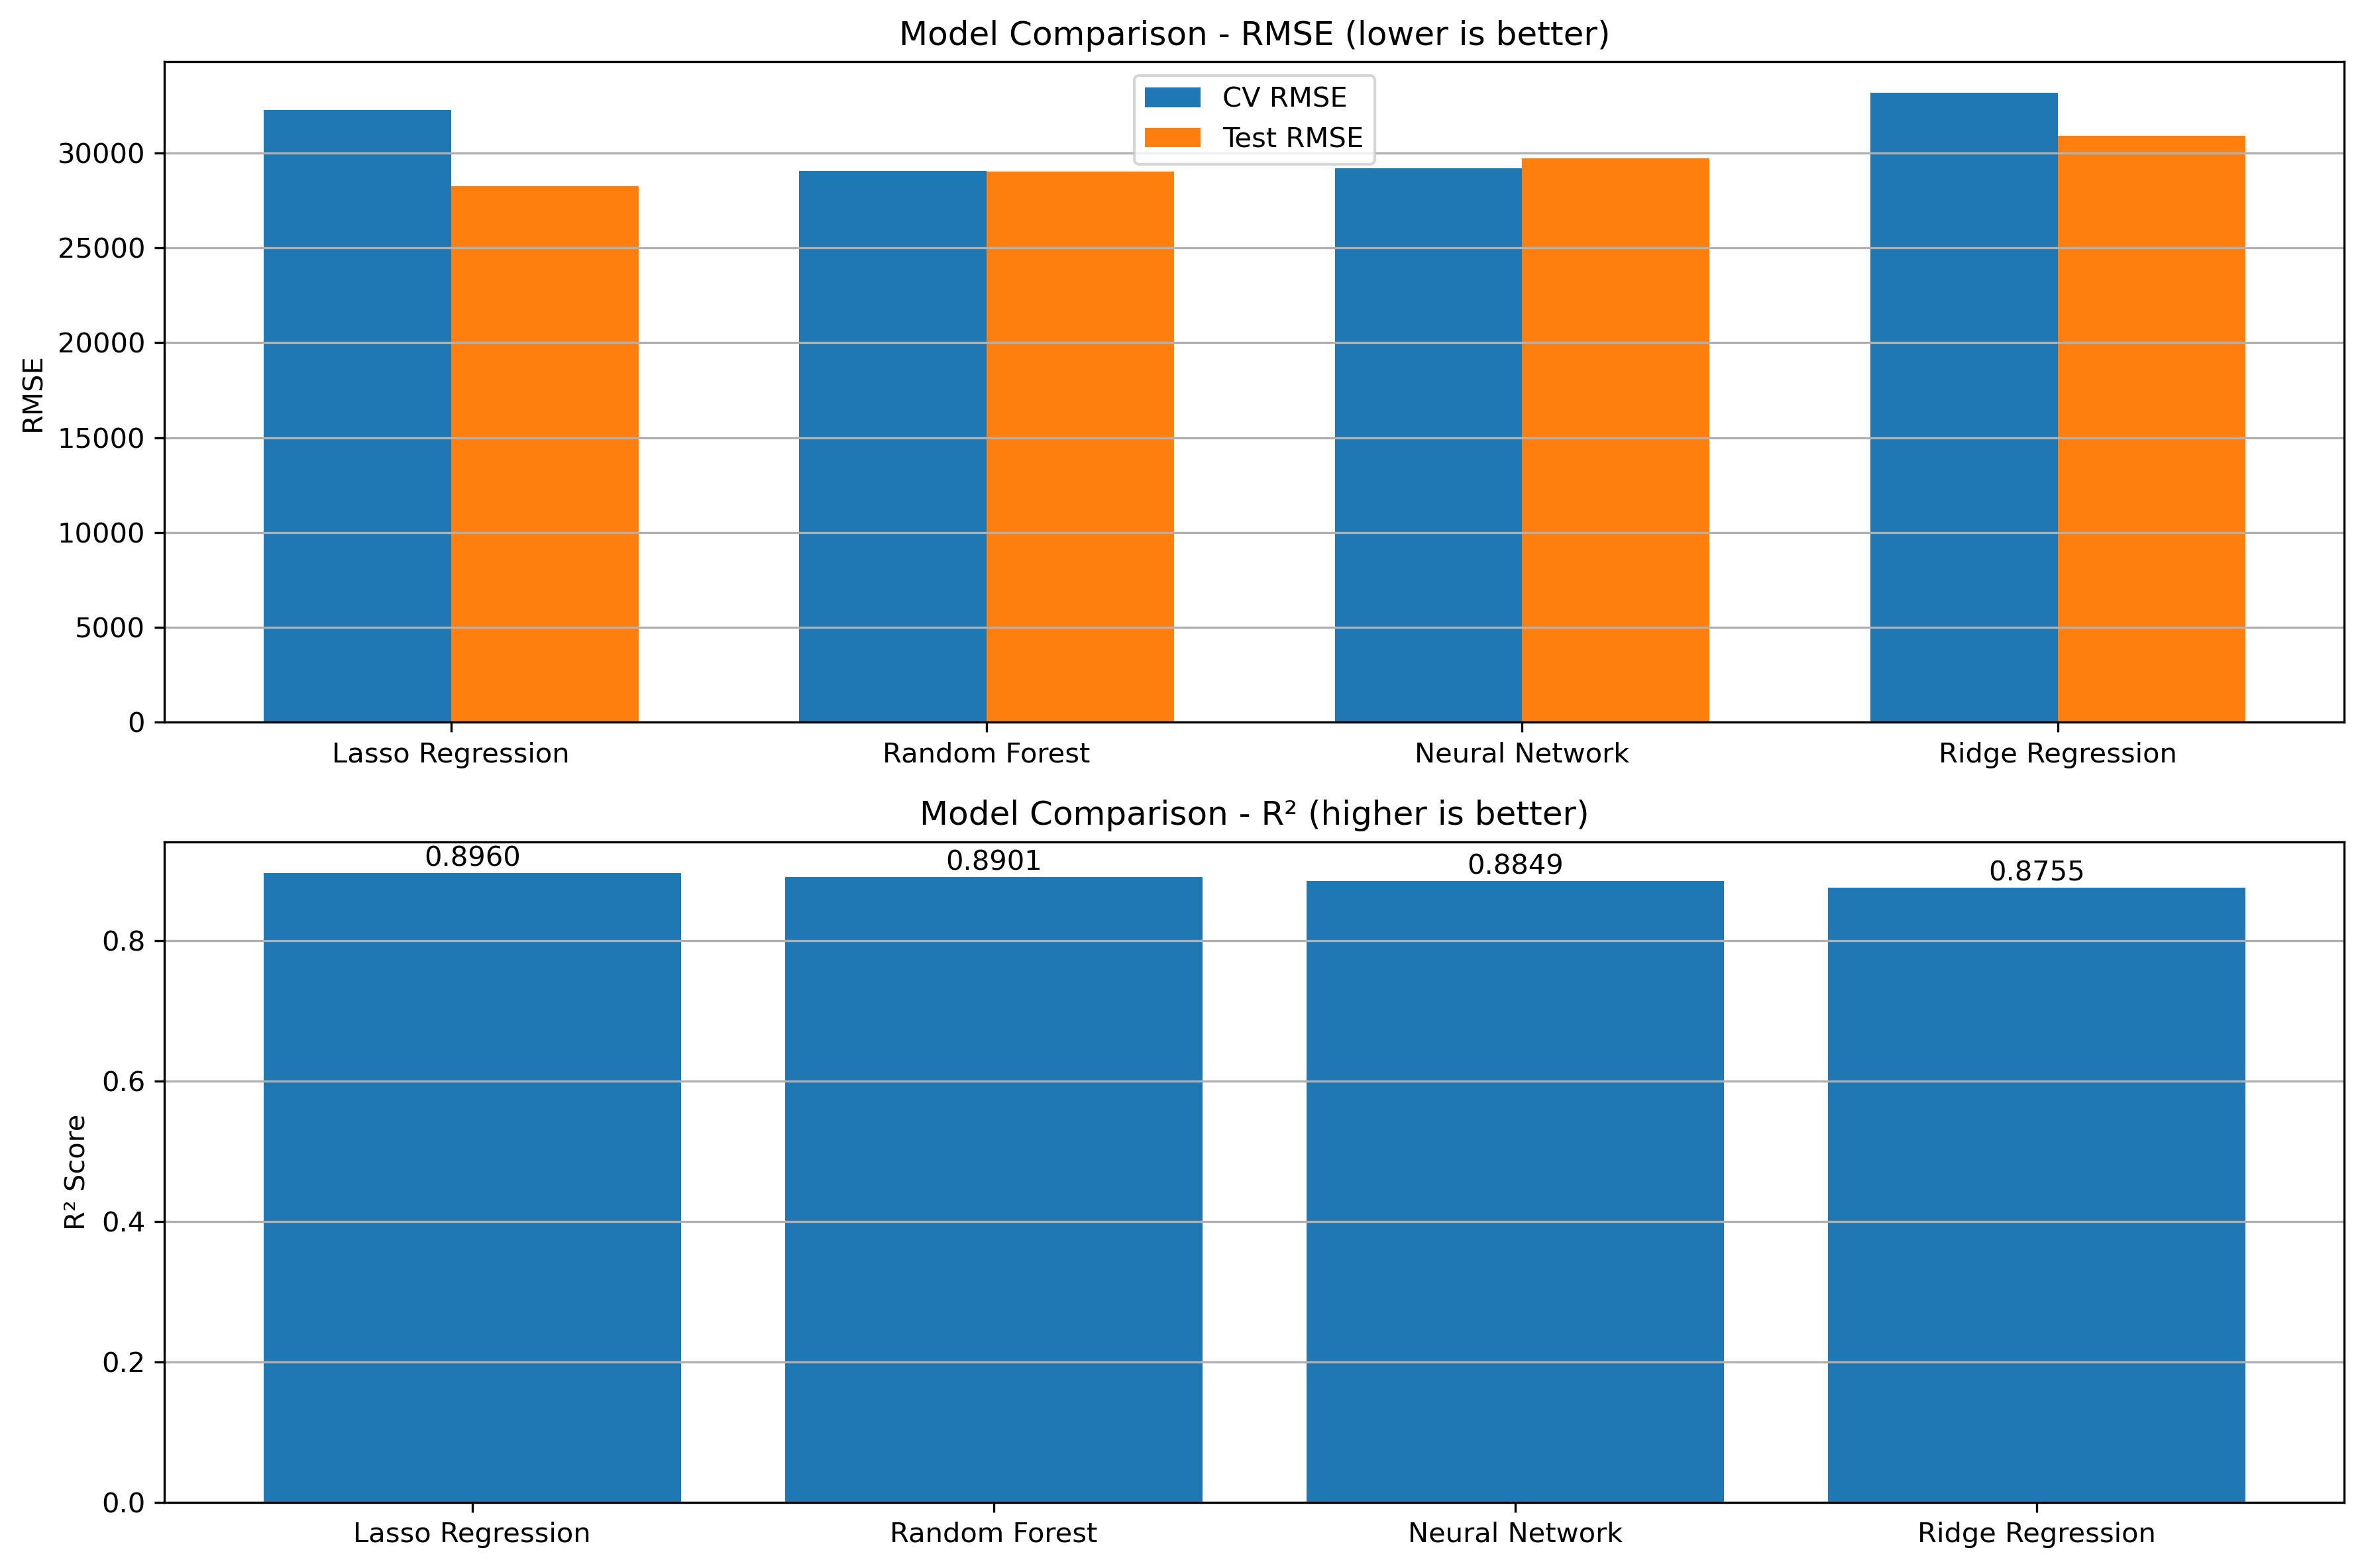
\includegraphics[width=1.0\textwidth]{figures/model_comparison.png}
    \caption{Performance Comparison Across All Four Models}
    \label{fig:model_comparison}
\end{figure}

Comparative analysis reveals several important insights:
\begin{itemize}
    \item \textbf{Lasso Regression} achieved the best overall performance with the lowest test RMSE (28,241.51) and highest R² (0.8960)
    \item \textbf{Random Forest} followed closely with test RMSE of 29,032.17 and R² of 0.8901
    \item \textbf{Ridge Regression} performed well but slightly behind the other two methods (RMSE: 30,907.81, R²: 0.8755)
    \item \textbf{Neural Network} significantly underperformed with extremely high RMSE and negative R²
\end{itemize}

These results highlight several key considerations for housing price prediction:
\begin{itemize}
    \item Linear models with proper regularization can perform remarkably well on this dataset
    \item Lasso's automatic feature selection provides an edge by creating a more parsimonious model
    \item Random Forest's ability to capture non-linear relationships makes it competitive
    \item Neural networks require more data and careful tuning to be effective for this type of problem
    \item Cross-validation provides reliable estimates of generalization performance
\end{itemize}

Performance differences between the top three models were relatively small, suggesting that any of these approaches could be viable in practice, with the choice depending on specific requirements for interpretability, feature selection, and implementation complexity.

\section{Key Findings and Recommendations}
Based on the comprehensive modeling analysis with four different approaches:
\begin{itemize}
    \item Ridge Regression:
    \begin{itemize}
        \item Best for handling multicollinearity
        \item Provides stable feature importance estimates
        \item Shows which features have the strongest linear relationship with price
        \item Good performance with RMSE of 30,907.81 and R² of 0.8755
    \end{itemize}
    \item Lasso Regression:
    \begin{itemize}
        \item Offers automatic feature selection
        \item Produces sparse solutions
        \item Identifies the most crucial predictors
        \item Best overall performance with RMSE of 28,241.51 and R² of 0.8960
    \end{itemize}
    \item Random Forest:
    \begin{itemize}
        \item Captures non-linear relationships and interactions
        \item Strong predictive performance (RMSE: 29,032.17, R²: 0.8901)
        \item Less sensitive to outliers and non-normal distributions
        \item Provides reliable feature importance measurements
    \end{itemize}
    \item Neural Network:
    \begin{itemize}
        \item Struggled with this dataset (negative R²)
        \item Requires more data and careful tuning
        \item Not recommended for this specific housing prediction task
        \item May benefit from more advanced architectures or ensemble approaches
    \end{itemize}
\end{itemize}

For practical implementation in real estate valuation applications, we recommend:
\begin{itemize}
    \item Use Lasso Regression when interpretability and model simplicity are important
    \item Consider Random Forest when capturing complex feature interactions is critical
    \item Employ Ridge Regression when dealing with highly correlated features
    \item Avoid neural networks for housing price prediction unless substantially more data is available
    \item Consider ensemble approaches combining the strengths of multiple models
\end{itemize}

\section{Future Improvements}
Potential enhancements for model performance:
\begin{itemize}
    \item Ensemble methods combining multiple models, particularly Lasso and Random Forest
    \item More sophisticated feature engineering based on domain knowledge
    \item Hyperparameter optimization through grid search or Bayesian optimization
    \item Integration of temporal market trends
    \item Neighborhood-specific sub-models
    \item For neural networks: 
    \begin{itemize}
        \item More extensive architecture search
        \item Advanced regularization techniques
        \item Feature preprocessing specific to neural networks
        \item Larger dataset collection
    \end{itemize}
\end{itemize} 